\section{User centered Design}

\begin{breakbox}
\boxtitle{Simplification}

The solution for bigger screens and better usability is \textbf{simplification}.

\begin{itemize}
    \item Remove features: Get rid of buttons that you never seem to use 
    \item Hide features: unimportant stuff, but harder to reach
    \item Group features: Move imporant stuff and group everything in logical groups
    \item Displace features: e.g.~move features in a on-screen menu
\end{itemize}

A good simplification is always targeted to a user group. For who is this simplification done? 
\end{breakbox}

\begin{breakbox}
\boxtitle{Simplification Context} \\
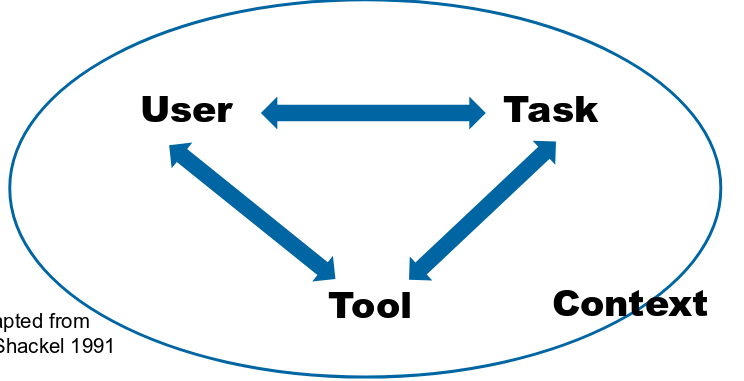
\includegraphics[width=.2\textwidth]{figures/simplification_context.png}
\end{breakbox}

\begin{breakbox}
\boxtitle{User Centered Design}

There is an ISO standard (ISO 9241 parts 110) for the definition of
usability and the evaluation of the product:

\begin{itemize}
\tightlist
\item
  Suitability for the task
\item
  Self descriptiveness
\item
  Controllability
\item
  Conformity with user expectations
\item
  Error tolerance
\item
  Suitability for individualization
\item
  Suitability for learning
\end{itemize}

The second part of this standard describes the user centered design
process.
\end{breakbox}

\begin{breakbox}
\boxtitle{User Centered Design Process} \\
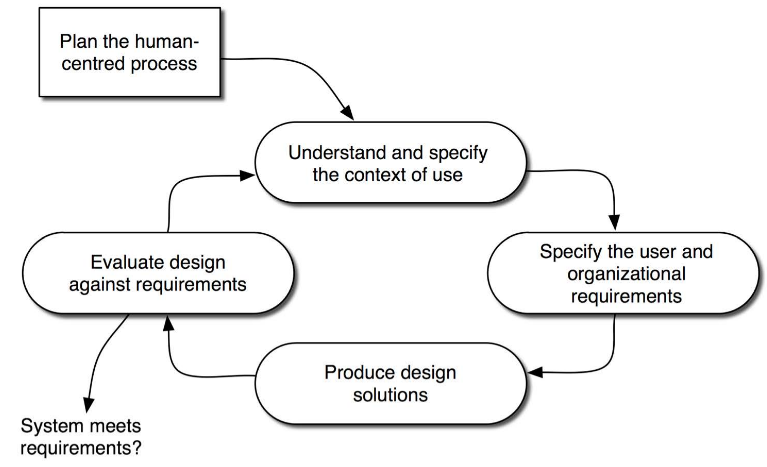
\includegraphics[width=.25\textwidth]{figures/standard_user_centered_process.png}
\end{breakbox}

\begin{breakbox}
\boxtitle{Who to ask?} \\
To design the best UX, \textbf{pay attention to what users do, not what they say}. Self-reported claims are unreliable, as are user speculations about future behavior. Users do not know what they want. You may ask your customers, but not your users

\textbf{The user is the problem expert}
\begin{itemize}
    \item He can be interviewed about encountered problems
    \item He might explain how things should be done, not how they are actually done
\item He should be observed doing current tasks
\item He can be asked to explain observed behavior
\end{itemize}

\textbf{The designer is the solution expert}
\end{breakbox}


\section{Scenarios}
\begin{breakbox}
\boxtitle{Why Scenarios?} \\
With scenarios, you are able to do a documentation of the user research
results. They provide a story of the user solving a problem. 
\begin{itemize}
    \item Problem-Scenarios show current (problematic) situations
    \item Future-Scenarios show users with the same needs and in a similar context
as in the problem-scenarios, but they illustrate how the new tools help.
\end{itemize}
\end{breakbox}

\begin{breakbox}
\boxtitle{First Success} 

\begin{itemize}
    \item Why (how, when) was the app
installed by user
\item Why is the app used the first time (trigger,
motivation to start, motivation to go through all the required steps
until success)
\item When is the first time (step) the user gets a
recognizable reward/benefit from the use of the app?
\end{itemize}

\end{breakbox}

\begin{breakbox}
\boxtitle{Repeated Success} 

\begin{itemize}
    \item Why is the user starting the
app again (trigger)?
\item  What are the repeated benefits?
\item How does the
app cater for expert users without loosing infrequent users?
\end{itemize}

\end{breakbox}

\columnbreak
\begin{breakbox}
\boxtitle{Repeated Success - Example} \\

\textbf{Persona:} \\
Bob Busy: Bread-lover, buys his bread from his local bakery, \\
Quote: "There are only few bread-types that I like. \\
Dinner without my favorite bread is a disaster." \\
\textbf{Context:} \\
Bob has been a regular user of the breadwinner app for over a month now.
It is Wednesday.
By tracking his usage patterns the Breadwinner app has determined that Bob likes to buy a
loaf St. Galler bread on Wednesday evenings. Shortly before noon the app generates a push
notification to ask whether Bob would like to reserve a loaf of St. Galler bread today. \\
\textbf{Trigger \& Steps:} \\
During his lunch beak Bob sees the notification and uses it to open the Breadwinner app.
The app immediately displays a "quick reservation" button along with todays opening hours
of Bob's local bakery. It also allows to reserve other types of bead and pastry. Bob quickly
pushes the the button to reserve "his" loaf of St Galler bread. He then closes the app.
At 6PM – Bob has just exited the train to return home -- he receives another notification
reminding him to pick up his reserved bread. He hurries to the bakery to pick up the loaf. At
the bakery he does not need to pay for the bread as the price is deduced from his pre-pay
account. He also takes an additional pastry that is offered as "special offer" to regular
customers \\
\textbf{The End / Solution:} \\
Bob enjoys his fresh favorite bread and pastry for dinner

\end{breakbox}

\begin{breakbox}
\boxtitle{Virality Scenario} 

\begin{itemize}
    \item Why (how) will the user tell others
about the app or get them involved?
\end{itemize}

\end{breakbox}

\section{BBV's How to build a great app}

\begin{breakbox}
\begin{itemize}
\tightlist
\item
  Define the purpose of your App (!)
\item
  Know your Target Group and Usage Context (!)
\item
  Reduce to the max:

  \begin{itemize}
  \tightlist
  \item
    Minimal (optimal) number of functions
  \item
    Minimal (optimal) amount of information on screens
  \end{itemize}
\item
  Optimize Navigation and User Guidance

  \begin{itemize}
  \tightlist
  \item
    Speak your users language
  \item
    Fast an fluent interaction
  \end{itemize}
\item
  Use Sensors to their Advantage
\item
  Professional Graphical Design
\item
  Adherer to Platform Guidelines
\item
  Marketing your App in the Appstore is a challenge
\end{itemize}

\end{breakbox}
